\documentclass[11pt,letterpaper]{article}
\usepackage[lmargin=1in,rmargin=1in,tmargin=1in,bmargin=1in]{geometry}
\usepackage{../style/homework}
\usepackage{../style/commands}
\setbool{quotetype}{true} % True: Side; False: Under
\setbool{hideans}{false} % Student: True; Instructor: False

% -------------------
% Content
% -------------------
\begin{document}

\homework{7: Due 03/01}{Life is a school of probability.}{Walter Bagehot}

% Problem 1
\problem{10} The probabilities of several events in a finite probability space are given below:
	\[
	\begin{aligned}
	P(A)&= 0.30 & P(B \text{ and } C)&= 0.15 \\
	P(B)&= 0.55 & P(D \;|\; A)&= 0.10 \\
	P(C)&= 0.75 & P(B \text{ and } D)&= 0.01 \\
	P(D)&= 0.25 & P(C \text{ and } D)&= 0.00
	\end{aligned}
	\] 
\begin{enumerate}[(a)]
\item Assuming that $A$ and $B$ are independent, find $P(A \text{ or } B)$.
\item Find $P(C \;|\; B)$.
\item Are $A$ and $C$ disjoint? Explain.
\item Are $B$ and $D$ independent? Explain. 
\item Find $P(A \text{ and } D)$. 
\end{enumerate} \pspace

\sol 
\begin{enumerate}[(a)]
\item Because $A$ and $B$ are independent, we know that $P(A \text{ and } B)= P(A) \cdot P(B)= 0.30 \cdot 0.55= 0.165$. But then we have\dots
	\[
	P(A \text{ or } B)= P(A) + P(B) - P(A \text{ and } B)= 0.30 + 0.55 - 0.165= 0.685
	\] \pspace

\item We have\dots
	\[
	P(C \;|\; B)= \dfrac{P(C \text{ and } B)}{P(B)}= \dfrac{P(C \text{ and } B)}{P(B)}= \dfrac{0.15}{0.55} \approx 0.2727
	\] \pspace

\item If $A$ and $C$ were disjoint, then $P(A \text{ or } C)= P(A) + P(C)$. But then $P(A \text{ or } C)= P(A) + P(C)= 0.30 + 0.75= 1.05$, which is impossible. Therefore, it is not possible for $A$ and $C$ to be disjoint. \pspace

\item If $B$ and $D$ were independent, then $P(B \text{ and } D)= P(B) \cdot P(D)$. We have $P(B \text{ and } D)= P(B) \cdot P(D)= 0.55 \cdot 0.25= 0.1375$. However, we know that $P(B \text{ and } D)= 0.01$. Because $0.1375 \neq 0.01$, we know that $B$ and $D$ are not independent. \pspace

\item We have\dots
	\[
	P(A \text{ and } D)= P(A) \cdot P(D \;|\; A)= 0.30 \cdot 0.10= 0.03
	\]
\end{enumerate}



\newpage



% Problem 2
\problem{10} At a small community college, the number of times students accessed tutoring resources available to them during a semester is summarized in the table below. \par
	\begin{table}[!ht]
	\centering
	\begin{tabular}{|l||c|c|c|c||c|} \hline
	& Never & 1 -- 2 & 3 -- 5 & > 5 & Total \\ \hline \hline
	Freshman & 72 & 86 & 45 & 17 & 220 \\ \hline
	Sophomore & 93 & 32 & 55 & 41 & 221 \\ \hline
	Junior & 63 & 44 & 46 & 19 & 172 \\ \hline
	Senior & 97 & 9 & 15 & 11 & 132 \\ \hline \hline
	Total & 325 & 171 & 161 & 88 & 745 \\ \hline
	\end{tabular}
	\end{table} \par
Based on the table above and showing all your work, answer the following:
\begin{enumerate}[(a)]
\item Find the probability that a randomly selected student never went to tutoring.
\item Find the probability that a randomly selected student is a Junior.
\item Find the probability that a randomly selected student went to tutoring once to two times or was a Sophomore. 
\item Find the probability that a randomly selected Senior went to tutoring more than five times. 
\item If a student was a Freshman, find the probability that they went to tutoring at most five times. 
\end{enumerate} \pspace

\sol We first need to find the totals for each row/column, which we include below on the table above.  
\begin{enumerate}[(a)]
\item We have\dots
	\[
	P(\text{no tutoring})= \dfrac{325}{745}= \dfrac{65}{149} \approx 0.4362
	\] \pspace

\item We have\dots
	\[
	P(\text{Junior})= \dfrac{172}{745} \approx 0.2309 
	\] \pspace

\item We have\dots
	\[
	\hspace{-1.5cm} P(\text{Tutoring 1 -- 2 or Sophomore})= \dfrac{86 + 32 + 44 + 9 + 93 + 55 + 41}{745}= \dfrac{171 + 221 - 32}{745}= \dfrac{360}{745}= \dfrac{72}{149} \approx 0.4832
	\] \pspace

\item We have\dots
	\[
	P(\leq 5 \;|\; \text{Senior})= \dfrac{P(\leq 5 \text{ and Senior})}{P(\text{Senior})}= \dfrac{97 + 9 + 15}{132}= \dfrac{121}{132}= \dfrac{11}{12} \approx 0.9167
	\] \pspace

\item We have\dots
	\[
	P(\leq 5 \;|\; \text{Freshman})= \dfrac{P(\leq 5 \text{ and Freshman})}{P(\text{Freshman})}= \dfrac{72 + 86 + 45}{220}= \dfrac{203}{220} \approx 0.9227
	\]
\end{enumerate} 



\newpage



% Problem 3
\problem{10} At a local car dealership, there are 460 cars in the lot. Of these cars, 45 of them are electric vehicles and 126 of them are SUVs. There are also 3 which are electric SUVs. 
	\begin{enumerate}[(a)]
	\item Find the probability that a randomly selected car was an electric vehicle. 
	\item Find the probability that a randomly selected car was an electric vehicle or an SUV.
	\item Find the probability that a randomly selected car was neither an electric vehicle nor an SUV.
	\item If a randomly selected car was an SUV, what is the probability that it was electric? 
	\item Find the probability that a randomly selected car was a non-SUV, electric vehicle. 
	\end{enumerate} \pspace

\sol 
\begin{enumerate}[(a)]
\item We have\dots
	\[
	P(\text{electric})= \dfrac{42 + 3}{460}= \dfrac{45}{460}= \dfrac{9}{92} \approx 0.0978
	\] \pspace

\item We have\dots
	\[
	P(\text{electric or SUV})= \dfrac{42 + 3 + 123}{460}= \dfrac{45 + 126 - 3}{460}= \dfrac{168}{460}= \dfrac{42}{115} \approx 0.3652
	\] \pspace

\item We have\dots
	\[
	P(\text{not electric nor SUV})= \dfrac{460 - 45 - 126 + 3}{460}= \dfrac{292}{460}= \dfrac{73}{115} \approx 0.6348
	\] \pspace

\item We have\dots
	\[
	P(\text{electric} \;|\; \text{SUV})= \dfrac{P(\text{electric SUV})}{P(\text{SUV})}= \dfrac{3}{3 + 123}= \dfrac{3}{126}= \dfrac{1}{42} \approx 0.0238
	\] \pspace

\item We have\dots
	\[
	P(\text{non-SUV, electric})= \dfrac{42}{460}= \dfrac{21}{230} \approx 0.0913
	\]
\end{enumerate} \vfill

	\[
	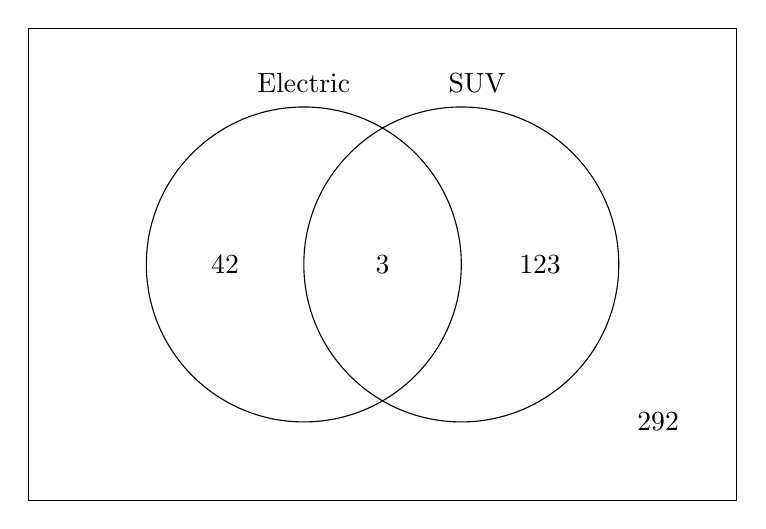
\begin{tikzpicture}
	\draw (0,0) rectangle (9,6);
	\draw (3.5,3) circle (2);
	\draw (5.5,3) circle (2);
	
	\node at (3.5,5.3) {Electric};
	\node at (5.7,5.3) {SUV}; 
	
	\node at (2.5,3) {42};
	\node at (4.5,3) {3};
	\node at (6.5,3) {123};
	\node at (8,1) {292};
	\end{tikzpicture}
	\]



\newpage



% Problem 4
\problem{10} You randomly assign delivery trucks routes to make their deliveries around the community. Of these routes, 40\% of them are highways, while the rest of them are surface streets. If a delivery truck takes the highway, they make their deliveries on-time 90\% of the time. If a delivery truck takes surface streets, they make their delivery on-time 85\% of the time.
	\begin{enumerate}[(a)]
	\item What percent of deliveries are on-time?
	\item What percent of deliveries are on-time or use surface streets?
	\item What percent of deliveries use highways?
	\item What percent of deliveries that use the highway are on-time?
	\item What percent of deliveries that are on-time use the highway?
	\end{enumerate} \pspace

\sol 
\begin{enumerate}[(a)]
\item We have\dots
	\[
	P(\text{on-time})= 0.36 + 0.51= 0.87
	\] \pspace

\item We have\dots
	\[
	P(\text{on-time or surface street})= 0.36 + 0.51 + 0.09= 0.96
	\] \pspace

\item We have\dots
	\[
	P(\text{highways})= 0.36 + 0.04= 0.40
	\] \pspace
	
\item We have\dots
	\[
	P(\text{on-time} \;|\; \text{highway})= \dfrac{P(\text{on-time and highway})}{P(\text{highway})}= \dfrac{0.36}{0.36 + 0.04}= \dfrac{0.36}{0.40} \approx 0.90
	\] \pspace

\item We have\dots
	\[
	P(\text{highway} \;|\; \text{on-time})= \dfrac{P(\text{highway and on-time})}{P(\text{on-time})}= \dfrac{0.36}{0.36 + 0.51}= \dfrac{0.36}{0.87} \approx 0.4138
	\]
\end{enumerate} \vfill

		\[
		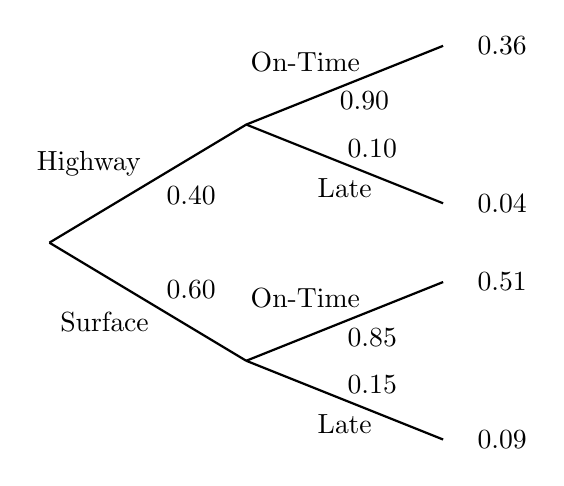
\begin{tikzpicture}[scale= 1.0]
		\def\FirstUpLabel{Highway}
		\def\FirstDownLabel{Surface}
		\def\SecondUpLabel{On-Time}
		\def\SecondDownLabel{Late}
		\def\Up{$0.40$}
		\def\Down{$0.60$}
		\def\UpUp{$0.90$}
		\def\UpDown{$0.10$}
		\def\DownUp{$0.85$}
		\def\DownDown{$0.15$}
		\def\first{$0.36$}
		\def\second{$0.04$}
		\def\third{$0.51$}
		\def\fourth{$0.09$}
		
		\node at (0.5,1) {\FirstUpLabel};	
		\node at (0.7,-1) {\FirstDownLabel};	
		\node at (1.8,0.6) {\Up};
		\node at (1.8,-0.6) {\Down};
		\draw[thick] (0,0) -- (2.5,1.5);
		\draw[thick] (0,0) -- (2.5,-1.5);
		
		\node at (3.25,2.3) {\SecondUpLabel};
		\node at (3.75,0.7) {\SecondDownLabel};
		\node at (4,1.8) {\UpUp};
		\node at (4.1,1.2) {\UpDown};
		\node at (5.75,2.5) {\first};
		\node at (5.75,0.5) {\second};
		\draw[thick] (2.5,1.5) -- (5,2.5);
		\draw[thick] (2.5,1.5) -- (5,0.5);

		\node at (3.25,-0.7) {\SecondUpLabel};
		\node at (3.75,-2.3) {\SecondDownLabel};
		\node at (4.1,-1.2) {\DownUp};
		\node at (4.1,-1.8) {\DownDown};
		\node at (5.75,-0.5) {\third};	
		\node at (5.75,-2.5) {\fourth};	
		\draw[thick] (2.5,-1.5) -- (5,-0.5);
		\draw[thick] (2.5,-1.5) -- (5,-2.5);
		\end{tikzpicture}
		\]


\end{document}